\chapter{Postprocessing methods for JICF}
\label{app:postproc_method_JICF}

\section{Jet trajectory}
\label{app:processing_JICF_trajectories}



Experimentally, researchers have used different approaches to obtain trajectories based on the different optical techniques employed. Many works \citemColor[becker_breakup_2002,stenzler_penetration_2003,freitag_spray_2008] take instantaneous images of the jet with shadowgraphy techniques and then MIE scattering or emboss-filter operations to obtain binary images where liquid and gas phases can be clearly distinguished. Then, images are averaged and the vertical penetration is obtained by detecting the coordinates where the light intensity gradients are maximum. Image averaging can be performed before or after the filtering operations. Such methods obtaining trajectories from average images are hereafter denoted as \textbf{mean trajectory methods}. Figure \ref{fig:expe_obtention_of_trajectories} shows an illustration of such experimental methodology from the work by \citeColor[stenzler_penetration_2003]. Other works \citepColor[ragucci_trajectory_2007] use the same principles of filtering and binarization, but obtain the trajectories from instantaneous jet images. Then, instantaneous trajectories are averaged to yield the mean trajectories. These methods are hereafter denoted as \textbf{instantaneous trajectory methods}.

\begin{figure}[ht]
     \centering
     \includeinkscape[inkscapelatex=false,scale=0.6]{./part2_developments/figures_ch5_resolved_JICF/trajectories_obtention/expe_obtention}
     \caption{Illustration of experimental procedure to obtain trajectories. Figures taken from \citeColor[stenzler_penetration_2003]}
      \label{fig:expe_obtention_of_trajectories}
\end{figure}

From a computational perspective, similar methodologies can be applied to obtain the jet trajectories from simulations. The same sequence of operations from Figure \ref{fig:expe_obtention_of_trajectories} for processing experimental images could be applied to numerical snapshots of the JICF. Nevertheless, the ACLS methodology presents the advantage that the interface is clearly defined with the $\psi$ function, and hence trajectories can be obtained with different methods without the need to use MIE scattering and binarization (steps 2 and 3 from Figure \ref{fig:expe_obtention_of_trajectories}). In this work, four methodologies to obtain the numerical trajectories from JICF resolved simulations are presented. As in the experimental classification previously suggested to obtain trajectories, these methodologies are also distinguished as \textbf{mean trajectory methods} or \textbf{instantaneous trajectory methods}, depending on whether they use the mean or instantaneous $\psi$ field respectively. Two methods for each category are detailed in this section.



\paragraph*{Mean trajectory methods}

One possibility to obtain mean trajectories is by using the mean field of the levelset function, $\overline{\psi}$. An example of a converged $\overline{\psi}$ field is shown in Figure \ref{fig:trajectory_obtention_mean_methods_c_d} left. This requires the accumulation of statistics over a certain time (instantaneous trajectories do not need statistics accumulation as long as the instantaneous $\psi$ field is available), but presents the advantage that the jet trajectory can be obtained with one single $\overline{\psi}$ field once convergence is achieved. In this category, two different methods are used: the \textbf{maximum gradient method} and the \textbf{iso-contour method}:


\begin{itemize}

	\item The \textbf{maximum gradient method} consists to obtain the maximum gradient of $\overline{\psi}$ in the vertical direction for each $x$ coordinate: $\max \left( \nabla_z | \overline{\psi} | \right)$. Figure \ref{fig:trajectory_obtention_mean_methods_c_d} center shows an example of a $\max \left( \nabla_z | \overline{\psi} | \right)$ contour. This method is more similar to the experimental methods presented in \citeColor[becker_breakup_2002], \citeColor[stenzler_penetration_2003] and \citeColor[freitag_spray_2008]: in these works, the jet trajectory is obtained as the contour of the maximum intensity gradient in the vertical direction of the mean jet (see Figure \ref{fig:expe_obtention_of_trajectories}).
	
	\item Trajectory as \textbf{iso-contour} of mean levelset field $\overline{\psi}$. This approach has been used to obtain JICF trajectories with simulations using a VOF methodology \citepColor[desclaux_experimental_2020]. In this work, several values for the iso-contour have been tested, and it has been found that the mean trajectories obtained are very sensitive to this value. Finally, a value of $\overline{\psi} = 0.01$ has been identified as the best contour to compare the resulting trajectories with the ones obtained with the rest of methods. Figure \ref{fig:trajectory_obtention_mean_methods_c_d} right shows an example of a an example of a $\overline{\psi} = 0.01$ contour.


\end{itemize}

\begin{figure}[ht]
     \centering
     \includeinkscape[inkscapelatex=false,scale=0.35]{./part2_developments/figures_ch5_resolved_JICF/trajectories_obtention/methods_c_d_and_mean_psi_field}
     \caption[Methods based on mean trajectories]{Methods based on mean trajectories. \textsl{Left}: $\overline{\psi}$ field. \textsl{Center}: $\max \left( \nabla_z | \overline{\psi} | \right)$ contour. \textsl{Right}: contour $\overline{\psi} = 0.01$.}
	% See: https://stackoverflow.com/questions/35210337/can-i-plot-several-histograms-in-3d/35225919
      \label{fig:trajectory_obtention_mean_methods_c_d}
\end{figure}

\vspace*{-0.2in}

\paragraph*{Instantaneous trajectory methods}

Instead of using the mean levelset field, the averaged numerical trajectories can be obtained from instantaneous solutions of the jet by firstly getting the instantaneous trajectories and then averaging them. Figure \ref{fig:trajectory_obtention_instantaneous_general} shows the procedure to extract the interface contour that is later used to obtain the trajectories. First, the liquid-gas interface is plotted in the domain as a surface of iso-contour $\Gamma: \psi = 0.5$ (Figure \ref{fig:trajectory_obtention_instantaneous_general} left), and then this contour is extracted at the central plane $y = 0$, as indicated by the black line of Figure \ref{fig:trajectory_obtention_instantaneous_general} right. 

\begin{figure}[h]
     \centering
     \begin{subfigure}[b]{0.45\textwidth}
         \centering
         \includeinkscape[inkscapelatex=false,scale=0.35]{./part2_developments/figures_ch5_resolved_JICF/trajectories_obtention/instantaneous_interface_3D}
         %\caption{Instantaneous jet interface}
     \end{subfigure}
     %\hfill
     \begin{subfigure}[b]{0.45\textwidth}
         \centering
         \includeinkscape[inkscapelatex=false,scale=0.35]{./part2_developments/figures_ch5_resolved_JICF/trajectories_obtention/instantaneous_interface_y0}
         %\caption{Contour of instantaneous interface at plane y = 0}
     \end{subfigure}
        \caption[Procedure to obtain instantaneous trajectories.]{Procedure to process instantaneous trajectories. \textsl{Left}: instantaneous jet interface. \textsl{Right}: contour of instantaneous interface at plane y = 0}
	% See: https://stackoverflow.com/questions/35210337/can-i-plot-several-histograms-in-3d/35225919
        \label{fig:trajectory_obtention_instantaneous_general}
\end{figure}

Once the interface is obtained at $y = 0$, the outer contour of the trajectory must be obtained. This is the one corresponding to the windward side of the jet, and hence the one defining the instantaneous trajectory. For its obtention, the $z$ axis is swept and the points belonging to the trajectory are obtained as follows:

\begin{enumerate}

	\item The $z$ axis is discretized in intervals with constant thickness.
	
	\item For each interval, the contour point with minimum $x$ coordinate is obtained.
	
	\item Points are sorted according to their $x$ coordinate, defining the trajectory.

\end{enumerate}

This procedure is repeated at every instantaneous snapshot of the jet to obtain the corresponding trajectories. Then, all  trajectories are interpolated in the same axial locations and averaged to yield mean trajectories which can be compared to experimental correlations. This method is similar to the experimental methodology employed by \citeColor[ragucci_trajectory_2007], and was used by \citeColor[leparoux_primary_2018] to simulate their experimental configuration and validate the computations. However, it differs from the methodology employed by \citeColor[becker_breakup_2002], whose experimental test rig is simulated in this work and who obtained the trajectories with a methodology more similar to the mean trajectory methods (see next point). Still, it is worth to investigate the instantaneous methodologies and to compare them with the mean methods to illustrate the effect that the post-processing methodology can have on the jet trajectories when treating the same simulations.

The procedure previously described works properly in the dense core, where the interface contour is continuous up to the breakup point $z_b$. After this location, atomization takes place and the detected interface contours belong to ligaments or droplets. In this case, the definition of \textsl{outer trajectory} does not hold as clearly as in the dense core: some contours detected might belong to satellite droplets or to drops originated from surface breakup, and could modify the final average trajectory by lowering it down. With this consideration, two different trajectories are distinguished in the instantaneous methodologies: \textbf{non-monotonic} and \textbf{monotonic} trajectories:

%\subsubsection*{Non-monotonic trajectory}

\begin{itemize}

	\item \textbf{Non-monotonic instantaneous trajectories} can be obtained by applying the methodology as explained in the previous lines, accounting also for the contours which a priori do not pertain to the instantaneous trajectory. This procedure is illustrated in Figure \ref{fig:trajectory_obtention_instantaneous_method_a}: the different points of the trajectory are obtained when sweeping the $z$ axis, and the instantaneous trajectory is obtained by joining these points. Then, sorting all the sampled points along the $x$ axis creates a non-monotonic trajectory since some contour points belong to liquid structures further downstream, see Figure \ref{fig:trajectory_obtention_instantaneous_method_a} right.



\item \textbf{Monotonic instantaneous trajectories} are obtained similarly to non-monotonic ones but with one fundamental difference: when sorting along the $x$ axis, only points with increasing $z$ coordinate are considered. In this way, a monotonic trajectory is obtained, see Figure \ref{fig:trajectory_obtention_instantaneous_method_b} right. 




\end{itemize}

Table \ref{tab:jicf_tools_trajectories_obtention} shows a summary of the four methodologies presented, and the names used in $\S$\ref{subsec:ch5_jet_trajectories_results} to display the results.

\clearpage

\begin{figure}[ht]
     \centering
     \begin{subfigure}[b]{0.45\textwidth}
         \centering
         \includeinkscape[inkscapelatex=false,scale=0.35]{./part2_developments/figures_ch5_resolved_JICF/trajectories_obtention/method_a_sweep_nonMonotonic}
         %\caption{Instantaneous jet interface}
     \end{subfigure}
     %\hfill
     \begin{subfigure}[b]{0.45\textwidth}
         \centering
         \includeinkscape[inkscapelatex=false,scale=0.34]{./part2_developments/figures_ch5_resolved_JICF/trajectories_obtention/method_a_inst_trajectory}
         %\caption{Contour of instantaneous interface at plane y = 0}
     \end{subfigure}
        \caption[Obtention of non-monotonic instantaneous trajectory]{Obtention of non-monotonic instantaneous trajectory. \textsl{Left}: sweep process along z axis of interface points. \textsl{Right}: instantaneous trajectory.}
	% See: https://stackoverflow.com/questions/35210337/can-i-plot-several-histograms-in-3d/35225919
        \label{fig:trajectory_obtention_instantaneous_method_a}
\end{figure}

\begin{figure}[ht]
     \centering
     \begin{subfigure}[b]{0.45\textwidth}
         \centering
         \includeinkscape[inkscapelatex=false,scale=0.35]{./part2_developments/figures_ch5_resolved_JICF/trajectories_obtention/method_b_sweep_monotonic}
         %\caption{Instantaneous jet interface}
     \end{subfigure}
     %\hfill
     \begin{subfigure}[b]{0.45\textwidth}
         \centering
         \includeinkscape[inkscapelatex=false,scale=0.33]{./part2_developments/figures_ch5_resolved_JICF/trajectories_obtention/method_b_inst_trajectory}
         %\caption{Contour of instantaneous interface at plane y = 0}
     \end{subfigure}
        \caption[Obtention of monotonic instantaneous trajectory]{Obtention of monotonic instantaneous trajectory. \textsl{Left}: sweep process along z axis of interface points, excluding points whose vertical location is lower than the vertical location of the previous ones. \textsl{Right}: instantaneous trajectory.}
	% See: https://stackoverflow.com/questions/35210337/can-i-plot-several-histograms-in-3d/35225919
        \label{fig:trajectory_obtention_instantaneous_method_b}
\end{figure}


% The two instantaneous methodologies described here will provide the same trajectories in the dense core, but will differ after the breakup point. Therefore, the trajectories obtained from this methodology can be compared and used to estimate an average position of the dense core. 










\section{Direct measurement of liquid fluxes}
\label{app:processing_JICF_IBS}

While for obtaining lagrangian quantities the droplets are tracked through the sampling planes when they cross their axial locations $x$, direct measurement of the fluxes requires the integration of the level-set function $\psi$ in all the mesh elements conforming the plane. Therefore, it is necessary to consider all the mesh elements that intersect with the defined sampling plane for the numerical computation of the fluxes. Figure \ref{fig:jicf_IBs_sketch_calculation} shows an example of a plane perpendicular to the crossflow with all the 3D elements intersecting this plane. This geometrical entity where fluxes are directly integrated will be hereafter referred as \textbf{interior boundary} (IB). 

\begin{figure}[ht]
     \centering
     \includeinkscape[inkscapelatex=false,scale=0.3]{./part2_developments/figures_ch5_resolved_JICF/jicf_IBs_sketch_calculation}
     \caption{Interior boundaries discretization for obtention of liquid flow rates.}
	% Right figure available in C:\Users\d601630\Desktop\Project related\CLOSED\2020\2020-09-30 - IBs flow rate expression obtention -> test_case.pptx
      \label{fig:jicf_IBs_sketch_calculation}
\end{figure}

Liquid flow rates can be calculated in the IBs from the levelset function $\psi$ by applying directly Eq. (\ref{eq:mass_flow_rate_definition_general}) divided by the density, with $\phi = \psi$:

\begin{equation}
\label{eq:Q_lIB_general_definition}
Q_{l,\mathrm{IB}} = \int_{\mathrm{IB}} \psi \left( \textbf{u} \cdot \textbf{n} \right) dS
\end{equation}


For evaluating this integral, firstly the liquid flux through each mesh element belonging to the IB is needed. As depicted in \ref{fig:jicf_IBs_sketch_calculation} right, each surface element is defined by a normal $n_e$ and by three nodes $N_\mathrm{no} = 3$. Physical quantities are stored at the nodes, so the liquid flux passing through each single element is calculated as:

\begin{equation}
Q_{l,e} = \frac{1}{N_\mathrm{no}} \sum_{i=1}^{N_\mathrm{no}} \psi_i \textbf{u}_i \textbf{n}_e
\end{equation}

Then, all elements are summed up to yield the liquid flux at the IB:

\begin{equation}
\label{eq:Q_lIB_definition_with_Ne_and_No}
Q_{l,\mathrm{IB}} = \sum_{e=1}^{N_e} Q_{l,e} = \sum_{e=1}^{N_e} \frac{1}{N_\mathrm{no}} \sum_{i=1}^{N_\mathrm{no}} \psi_i \textbf{u}_i \textbf{n}_e
\end{equation}

With this procedure, the instantaneous liquid flow rates at a given IB is obtained. Fluxes are then monitored with time and statistics (mean and RMS quantities) can be obtained. \\






In the same way as the sampled lagrangian spray can be in-plane characterized (see $\S$\ref{subsec:SLI_spatial_discretization}), liquid fluxes can also be spatially discretized in the IBs. The procedure is shown in Figure \ref{fig:jicf_IBs_sketch_discretization}: a grid composed of rectangular probes can be defined in the IB, so that all elements comprised by the probes are contained. However, it is observed that the rectangular mesh does not fully match the elements distributed in the IB, since the CFD mesh is not uniform and is comprised of tetrahedral elements. Therefore, the requested rectangular probes cannot be obtained in the IB, as it often crosses elements (red line in Figure \ref{fig:jicf_IBs_sketch_discretization} right). Instead, the probes used for calculation of spatially distributed fluxes are adjusted to take into account the elements that are crossed by the requested mesh, as indicated by the green line in Figure \ref{fig:jicf_IBs_sketch_discretization} right. Therefore, the actual probes used for calculation are not rectangular, but fitted to the actual mesh in order to properly retrieve fluxes. 


\begin{figure}[ht]
     \centering
     \includeinkscape[inkscapelatex=false,scale=0.2]{./part2_developments/figures_ch5_resolved_JICF/jicf_IBs_sketch_discretization}
     \caption{Interior boundaries discretization for obtention of bounded flow rates.}
	% See: https://stackoverflow.com/questions/35210337/can-i-plot-several-histograms-in-3d/35225919
      \label{fig:jicf_IBs_sketch_discretization}
\end{figure}










%\begin{figure}[ht]
%     \centering
%     \begin{subfigure}[b]{0.45\textwidth}
%         \centering
%         \includeinkscape[inkscapelatex=false,scale=0.35]{./part2_developments/figures_ch5_resolved_JICF/trajectories_obtention/instantaneous_interface_3D}
%         %\caption{Instantaneous jet interface}
%     \end{subfigure}
%     %\hfill
%     \begin{subfigure}[b]{0.45\textwidth}
%         \centering
%         \includeinkscape[inkscapelatex=false,scale=0.35]{./part2_developments/figures_ch5_resolved_JICF/trajectories_obtention/instantaneous_interface_y0}
%         %\caption{Contour of instantaneous interface at plane y = 0}
%     \end{subfigure}
%        \caption[Planes where fluxes are measured with interior boundaries.]{Planes where fluxes are measured with interior boundaries. \textsl{Left}: planes perpendicular to crossflow direction. \textsl{Right}: filming planes.}
%	% See: https://stackoverflow.com/questions/35210337/can-i-plot-several-histograms-in-3d/35225919
%        \label{fig:jicf_interior_boundaries_surface_measurements}
%\end{figure}
%




\section{Dense core breakup point}
\label{app:processing_JICF_DC_breakup_point}


\subsubsection*{Topology processing methodology}

The procedure to extract the DC, depicted in Figure \ref{fig:dense_core_extraction}, works as follows:

\begin{enumerate}

	\item \textbf{DC identification and isolation}. The DC is identified at a given time instant as the liquid structure with largest volume in the simulation. This can easily be done with YALES2 since each liquid structure has a unique tag, named droplet number, which helps to differentiate it from the others. The droplet number with the associated largest volume in the domain is isolated from the others, so the coordinates of the liquid nodes belonging to the dense core are obtained.
	
	\item \textbf{Topology characterization}. Once the DC has been obtained, its topology is characterized through its \textbf{breakup point} and \textbf{width}:
	
	\begin{itemize}
	
		%\item The breakup point ($x_b, z_b$) is obtained as the point at the symmetry plane $y = 0$ with is located further in the streamwise direction $x$. 
	
		\item The breakup point ($x_b, z_b$) is obtained as the point at the symmetry plane $y = 0$ which is located further away from the injection location in the vertical direction $z$.
		
		\item The width $w$ is obtained by sweeping the DC along the $x$ axis and discretizing it into segments of size $\Delta x$. For each segment, the maximum and minimum points in the $y$ direction are calculated, i.e. the points which are located further away from the symmetry plane at both sides of the jet in a $x-y$ plane. The difference between this maximum and minimum denote the local width at each segment: the DC width is obtained as the maximum value of all the local widths obtained.
	
	\end{itemize}
	
\end{enumerate}

\begin{figure}[ht]
     \centering
     \includeinkscape[inkscapelatex=false,scale=0.20]{./part2_developments/figures_ch5_resolved_JICF/dense_core_extraction}
     \caption{Extraction of dense core from resolved atomization simulations.}
     % La solucion es UG75_DX10, r21 sol33
      \label{fig:dense_core_extraction}
\end{figure}

The DC is then characterized by its breakup point coordinates ($x_b, z_b$) and its width $w$. These values are time-dependent, and therefore statistics will be obtained from them. It is also important to note that the procedure employed to extract the DC from YALES2 simulations is ad-hoc and is not based on any methodology employed in experimental works to characterize the DC. This is justified by the fact that there are not many experimental studies on the JICF topology and not one single one of them applies to the operating conditions studied in this work. Therefore, no proper experimental validation can be performed for the DC characteristics. Instead, the main purpose of this analysis is to obtain input values for the ALM employed in lagrangian simulations.

\subsubsection*{Net force obtention}
%\label{subsec:ch5_force_determination_JICF}


Besides the dense core geometry, the net force $|\textbf{F}_\mathrm{DC}|$ needs also to be provided as input parameter to the ALM model. As explained in $\S$\ref{subsec:ch4_ALM_forces_determination}, the model considers only the contribution of the pressure momentum term and the force is calculated through Eq. (\ref{eq:ALM_Fp_calculation_simplified}). Two parameters are therefore needed: the dense core surface $S_\mathrm{DC}$ and the mean pressures in the windward and leeward sides. The surface is estimated through the mean values of the geometric dense core parameters, assuming that this one is a trapezoid with bases $d_\mathrm{inj}$, $\overline{w}$ and length $L_\mathrm{DC} = \sqrt{\overline{x_b}^2 + \overline{z_b}^2}$:

\begin{equation}
S_\mathrm{DC} = \frac{\left( d_\mathrm{inj} + \overline{w} \right) L_\mathrm{DC} }{2} 
\end{equation}

For estimating the mean pressures, the procedure schematized in Figure \ref{fig:extraction_methodology_mean_DC} is followed. First, the mean dense core is extracted from the resolved simulations as an iso-surface of the mean levelset surface: $\overline{\psi} = 0.5$. Then, the gradient vector $\nabla \left( \overline{\psi} \right)$ field is calculated on this surface, which points towards the direction of increasing values: that is, towards the inner part of the dense core, where $\overline{\psi} = 1$ in the areas where there is always liquid. The windward side of the mean dense core is then obtained as the region with a positive normal component of the gradient in the $x$ direction: $\nabla_x \left( \overline{\psi} \right) > 0$. Equivalently, the leeward side is defined by the points where $\nabla_x \left( \overline{\psi} \right) < 0$. Then, the mean pressure at both the windward and leeward sides, $p_\mathrm{windward}$ and $p_\mathrm{leeward}$ respectively, are calculated and taken as inputs to Eq. (\ref{eq:ALM_Fp_calculation_simplified}).

 
\clearpage

\begin{figure}[ht]
\centering
\includeinkscape[inkscapelatex=false,scale=0.33]{./part2_developments/figures_ch5_resolved_JICF/pressure_obtention_mean_DC/extraction_methodology_mean_DC}
\caption[Methodology to obtain windward and leeward surfaces of mean dense core from resolved atomization simulations]{Methodology to obtain windward and leeward surfaces of mean dense core from resolved atomization simulations. The displayed dense core corresponds to case UG100\_DX10.}
\label{fig:extraction_methodology_mean_DC}
\end{figure}

%Figure \ref{fig:jicf_DC_p_mean_scatterplots} shows scatterplots of the mean pressures obtained in the wind and leeward sides of the mean dense core projected in the $x-y$ plane. Pressures are positive in the windward side, the highest values being found in the central region close to the injector: here, the liquid column is mainly vertical and slightly deformed from a circular cross-section, hence the pressure exerted by the air is higher than at the top where the column starts deviating towards the crossflow direction (see Figure \ref{fig:extraction_methodology_mean_DC}). In the leeward side, the values are negative and minimum around the injector, while they increase upstream the dense core as its cross-section gets deformed. 


%\begin{figure}[ht]
%\flushleft
%\begin{subfigure}[b]{0.45\textwidth}
%	\flushleft
%   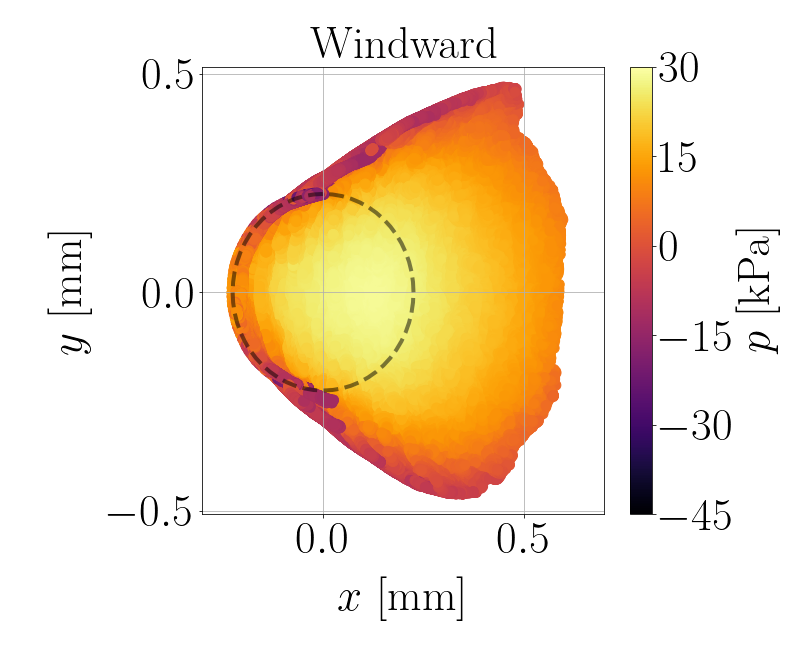
\includegraphics[scale=0.25]{./part2_developments/figures_ch5_resolved_JICF/pressure_obtention_mean_DC/p_mean_scatter_UG100_DX10_windward}
%   %\label{} 
%\end{subfigure}
%\hspace{0.5in}
%\begin{subfigure}[b]{0.45\textwidth}
%	\flushleft
%   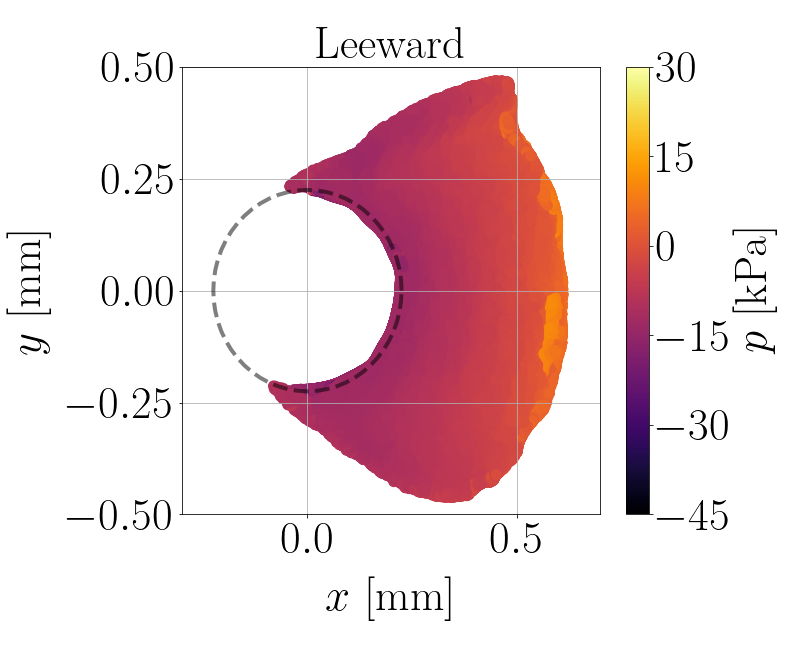
\includegraphics[scale=0.25]{./part2_developments/figures_ch5_resolved_JICF/pressure_obtention_mean_DC/p_mean_scatter_UG100_DX10_leeward}
%   %\label{}
%\end{subfigure}
%\caption[Projection of the windward and leeward surfaces in the $x-y$ plane colored by $\overline{p}$.]{Projection of the windward and leeward surfaces in the $x-y$ plane colored by $\overline{p}$. The dashed circumference denotes the injection nozzle.}
%\label{fig:jicf_DC_p_mean_scatterplots}
%\end{figure}




